\chapterimage{Water1.png} % Chapter heading image

\chapter{Drinking Water Regulations}

\begin{table}[H]
\begin{tabular}{| m{1cm} | m{15cm} |}
\hline
\multicolumn{2}{|l|}{\textbf{Expected   Range of Knowledge for Water Properties and Sources}}                                                                          \\ \hline
\multicolumn{2}{|l|}{\textit{Water   Distribution System Operator License Exams}}                                                                                      \\ \hline
D1 & Ability to read   a sample siting plan                                                                                    \\ \hline
D1 & Ability to take a   lead and copper sample                                                                                \\ \hline
D1 & Knowledge of acute   violations                                                                                           \\ \hline
D1 & Knowledge of CDPH   Water Quality regulations                                                                             \\ \hline
D1 & Knowledge of the   definition of MCL                                                                                      \\ \hline
D1 & Knowledge of the   major components of the SDWA                                                                           \\ \hline
D1 & Knowledge of the   purpose of the SDWA                                                                                    \\ \hline
D1 & Knowledge of Total   Coliform Rule reporting requirements                                                                 \\ \hline
D1 & Knowledge of Total   Coliform Rule sampling requirements                                                                  \\ \hline
D1 & Knowledge of when   public notification is required                                                                       \\ \hline
D2 & Ability to   differentiate between a primary and secondary MCL                                                            \\ \hline
D2 & Ability to recognize   MCL violations                                                                                     \\ \hline
D2 & Knowledge of AWWA   disinfection standards                                                                                \\ \hline
D2 & Knowledge of   Disinfection By-Product Rule sampling requirements                                                         \\ \hline
D2 & Knowledge of maximum   disinfectant residual level for chlorine                                                           \\ \hline
D2 & Knowledge of   reporting and recordkeeping requirements                                                                   \\ \hline
D3 & Knowledge of the   relationship between corrosion and lead/copper concentrations                                          \\ \hline
D3 & Knowledge of   Disinfection By-Product Rule MCL requirements                                                              \\ \hline
D3 & Knowledge of   Disinfection By-Product Rule reporting requirements                                                        \\ \hline
D3 & Knowledge of lead and   copper rule reporting requirements                                                                \\ \hline
D3 & Knowledge of lead and   copper sampling requirements                                                                      \\ \hline
D3 & Knowledge of public   notification requirements                                                                           \\ \hline
D3 & Ability to perform   damage assessment and recovery planning                                                              \\ \hline
D3 & Ability to train   personnel on emergency response procedures                                                             \\ \hline
D3 & Knowledge of   non-compliance penalties                                                                                   \\ \hline

\end{tabular}
\end{table}


\newpage



\begin{table}[H]
\begin{tabular}{| m{1cm} |m{15cm} |}
\hline
\multicolumn{2}{|l|}{\textbf{Expected   Range of Knowledge for Water Properties and Sources}}                                                                      \\ \hline
\multicolumn{2}{|l|}{\textit{Water   Distribution System Operator License Exams (Continued)}}                                                                  \\ \hline
D4 & Ability to recognize a lead and copper rule   violation                                                                   \\ \hline
D4 & Knowledge of notification paths (e.g.   newspaper, electronic)                                                            \\ \hline
D4 & Knowledge of required language to use                                                                                     \\ \hline
D5 & Knowledge of Air   Quality Management regulations                                                                         \\ \hline
D5 & Knowledge of O\&M   budget components (e.g. labor, professional services, supplies, energy,   water, capital improvement) \\ \hline
D5 & Knowledge of RWQCB   discharge requirements                                                                               \\ \hline
D5 & Knowledge of the   components of a budget (e.g. revenues, expenditures, risk management,   insurance costs, depreciation) \\ \hline
\multicolumn{2}{|l|}{\textit{Water   Treatment System Operator License Exams }}                                                                  \\ \hline
T1 & Knowledge of   disinfection residual requirements                                                                         \\ \hline
T1 & Knowledge of MCLs and   MRDLs of disinfectants                                                                            \\ \hline
T1 & Knowledge of drinking   water monitoring and reporting requirements                                                       \\ \hline
T1 & Knowledge of drinking   water regulations                                                                                 \\ \hline
T1 & Knowledge of   notification protocol and procedures                                                                       \\ \hline
T1 & Knowledge of NSF   Standards                                                                                              \\ \hline
T1 & Knowledge of operator   certification requirements                                                                        \\ \hline
T1 & Knowledge of Primary   and Secondary Drinking Water Standards                                                             \\ \hline
T1 & Knowledge of public   notification procedures                                                                             \\ \hline
T1 & Knowledge of record   keeping requirements                                                                                \\ \hline
T1 & Knowledge of   California Waterworks Standards                                                                            \\ \hline
T1 & Knowledge of the   Consumer Confidence Report (CCR)                                                                       \\ \hline
T1 & Knowledge of the   Disinfectants and Disinfection Byproduct Rule and amendments                                           \\ \hline
T1 & Knowledge of the   Groundwater Rule                                                                                       \\ \hline
T1 & Knowledge of the Lead   and Copper Rule                                                                                   \\ \hline
T1 & Knowledge of the   Surface Water Treatment Rule and amendments                                                            \\ \hline
T1 & Knowledge of the   Total Coliform Rule and amendments                                                                     \\ \hline
T1 & Ability to research   and interpret Maximum Contaminant Levels (MCLs)                                                     \\ \hline
T2 & Knowledge of   cryptosporidium action plan                                                                                \\ \hline
T2 & Knowledge of pending   regulations                                                                                        \\ \hline
T2 & Knowledge of   performance standards and removal requirements for surface water treatment                                 \\ \hline
T2 & Knowledge of the   Filter Backwash Rule                                                                                   \\ \hline
T2 & Knowledge of routine   sampling requirements                                                                              \\ \hline
T3 & Ability to administer   a regulatory compliance program                                                                   \\ \hline
T3 & Knowledge of permit   requirements for water operations                                                                   \\ \hline
T3 & Knowledge of pump to   waste discharge environmental regulations                                                          \\ \hline
T3 & Knowledge of   regulatory primacy issues                                                                                  \\ \hline
T3 & Knowledge of source   water replenishment processes                                                                       \\ \hline
T3 & Knowledge of the   Sanitary Survey process                                                                                \\ \hline
T4 & Knowledge of the role   of Regional Boards in managing contamination sources                                              \\ \hline
T4 & Knowledge of the   Source Water Assessment Program                                                                        \\ \hline
T4 & Knowledge of the   Watershed Survey process                                                                               \\ \hline
T4 & Knowledge of the   vulnerability assessment process                                                                       \\ \hline
\end{tabular}
\end{table}


\newpage






















\section{Drinking water regulations}\index{Drinking water regulations}
\begin{itemize}
\item Drinking water sources which include surface and groundwater sources have inherent vulnerabilities to contamination and regulations have been established to protect public health and safety.
\item Federal Safe Drinking Water Act (\textbf{SDWA}) \index{Safe Drinking Water Act (SDWA)} enacted in 1974 established national enforceable standards for drinking water quality and to guarantee that public water systems monitor water to ensure that it meets national standards. \\
\item The SDWA prescribes enforceable primary standards for five major categories of drinking water contaminants consisting of Inorganic Chemicals, Organic Chemicals, Radionuclides, Microorganisms, Disinfectants and Disinfection Byproducts.
\item The SDWA delegates responsibility for administering the provisions of
the act to the US Environmental Protection Agency (\textbf{USEPA}) \index{US Environmental Protection Agency (USEPA)}.
\item The enforcement of SDWA requirements is delegated by the USEPA to individual states
\item Individual states are provided the opportunity to set and enforce their own drinking water standards for public water systems if the standards are at a minimum as stringent as EPA's national standards.
\item A \textbf{primacy agency}is the agency with primary responsibility for implementing the SDWA. Most states and the U.S. territories have been approved to exercise primary responsibility in their jurisdictions. Exceptions are the state of Wyoming and the District of Columbia, which are implemented by EPA. 
\item In the SDWA, a \textbf{Public Water System} \index{Public water system}is defined as a system that supplies piped water for human consumption and has \textsl{\underline{at least 15 service connections or serves 25 or more persons for}}\\
\textsl{\underline{60 or more days of the year}}.\\
\textbf{Community Water System}\\
A community water system \index{Public water system!Community water system (CWS)} is a public water system \textsl{\underline{that has 15 or more service}}\\
\textsl{\underline{connections and is used by year-round residents or serves 25 or more residents year round}}.  These include city, county, regulated utilities \textsl{\underline{where people live}}.\\
\textbf{Non-Community Water System} \index{Public water system!Non-community water system (NCWS)} \\
Non-community water system means a public water system that is not a community water system. These are systems \textsl{\underline{with 15 or more connections used by travelers or intermittent users}}\\
\textsl{\underline{at least 60 days of a year or serves a daily average of at least 25 persons at least 60 days a year}}.
A non-community water system can be either:\\
\textbf{Transient Non-Community Water System} \index{Public water system!Transient non-community water system }\\
Include entities like rural gas stations and National parks that provide their own potable water source.  Here most people that consume the water neither reside nor regularly spend time there.\\
\begin{center}
OR\\
\end{center}
\textbf{Non-Transient Non-Community Water System} \index{Public water system!Water systems!Non-transient non-community water system }\\
Non-transient non-community water system means a public water system that is not a community water system and that regularly serves at least \textsl{\underline{25 of the same persons over six months}}\\
\textsl{\underline{per year}}.  These include places schools and businesses that provide their own water and the same people have a regular opportunity to consume the water, but do not reside there.
\item Water systems operated by private homes, groups of fewer than 15 homes using the same well, and summer camps that operate for fewer than 60 days per year are not covered under the purview of the SDWA but are generally under some degree of supervision by a local, area, or state health department.
\item Water treatment standards are set and enforced by the state’s nine regional water quality control boards in consultation with the California Department of Public Health. The nine regional boards are part of the State Water Board.
\end{itemize}

\subsection{National Primary Drinking Water Regulations}\index{National Primary Drinking Water Regulations}
\begin{itemize}
\item National Primary Drinking Water Regulations (\textbf{NPDWR}) \index{Safe Drinking Water Act (SDWA)!National Primary Drinking Water Regulations} is for contaminants – chemicals and microorganisms - found in drinking water and known to present adverse health effects to humans.
\item The contaminants are divided into two groups based upon its effect on human health:
\begin{enumerate}
\item \textbf{Acute} - effects occur within hours or days of the time a person consumes a contaminant
\item \textbf{Chronic} - effects occur over the course of many years after people consume a contaminant at levels over EPA's safety standards. 
\end{enumerate}
\item NPDWR are legally enforceable drinking water standards.  
\item The NPDWR standard can be either:
\vspace{0.3cm}
\begin{enumerate}
\item Maximum Contaminant Levels (\textbf{MCLs}) \index{Maximum contaminant levels (MCLs)} - the maximum permissible level of a contaminant in water which is delivered to any user of a public water system,  or 

\item Treatment technique which is a drinking water treatment requirement typically used when setting an MCL would be too difficult or when compliance with an MCL would be too costly.
\end{enumerate}
\item Additionally, Maximum Contaminant Level Goal (\textbf{MCLG})\index{Maximum contaminant level goal (MCLG)} - the maximum level goal is set at a level where there are no known, or anticipated health effects.  For suspected carcinogens and other similar contaminants, the MCLG is set at zero.
\item Drinking water must be monitored to ensure that it meets all applicable MCLs. Recurring sampling every three-years is stipulated.
\item The 90 Primary Contaminants identified by the EPA are grouped into three major categories:
\begin{enumerate}
\item Chemical contaminants
\begin{itemize}
\item Inorganic chemicals
\begin{itemize}
\item These contaminants are mostly heavy metals. 
\item They may enter the water supply naturally through groundwater formations or from mining runoff and industrial discharges.
\item Nitrates are the only chemical contaminant that represent an immediate health risk. Pregnant mothers and infants under 18 months can develop infant methemoglobinemia, commonly known as “Blue Baby Syndrome” \index{Blue baby syndrome/Infant methemoglobinemia} . The presence of nitrates in the bloodstream reduces oxygen uptake that gives the skin a blue tint.
\end{itemize}
\item Organic chemicals
\begin{itemize}
\item These contaminants include herbicides and insecticides that are primarily used in agriculture applications, organic solvents used in industrial applications, organic by-products of industrial processes, and chemical by- products from chlorination of drinking water.
\item Runoff from agricultural spraying or improper application techniques can be a major source of these contaminants in a surface water supply.
\item Industrial discharges, accidental spills and improper disposal of hazardous wastes can also become sources of contamination.
\item These compounds are grouped together under the headings of Volatile Organic Compounds (\textbf{VOCs}) and Synthetic Organic Compounds (\textbf{SOCs}). 

\item There are currently 21 regulated VOCs and 30 SOCs that must be analyzed.
\end{itemize}
\item The chemical contaminants were promulgated in phases collectively called the Phase II/V Rules or the Chemical Contaminant Rules.
\end{itemize}
\item Radioactive chemicals
\begin{itemize}
\item Most radioactive substances occur naturally in groundwater and in some surface supplies. 
\item Some man-made substances may also enter drinking water supplies from processing facilities, mining areas, and nuclear power plants. 
\end{itemize}

\item Bacteriological contaminants
\begin{itemize}
\item The coliform group of bacteria represents the indicator organisms used in determining bacteriological contamination. Their presence indicates the possibility that some pathogenic (disease causing) organisms may also be present. 
\item A public water system is in violation of the E. coli MCL when any of the following occurs:
\begin{enumerate}
\item The system has an E. coli-positive repeat sample following a total coliform-positive routine sample;
\item The system has a total coliform-positive repeat sample following an E. coli-positive routine sample;
\item The system fails to take all required repeat samples following an E. coli-positive routine sample; or
\item The system fails to test for E. coli when any repeat sample tests positive for total coliform.
\end{enumerate}
\item The MCL is exceeded when 5\% of the required monthly routine (M/R) samples indicate the presence of Coliform bacteria. 
\item The presence of coliform in any sample will require three repeat samples be taken. These repeat samples must be taken within 24 hrs of notification of positive results.
\end{itemize}
\end{enumerate}
\item Turbidity - Measure of the cloudiness of water. 
\begin{itemize}
\item Although turbidity does not represent a health risk by itself, it can shield harmful bacteria from disinfection processes.
\item Turbidity is measured in Nephelometric Turbidity Units (\textbf{NTU}) . 
\item The device used to measure NTU’s is called a nephelometer or turbidimeter.
\end{itemize}
\end{itemize}
\subsection{Secondary Drinking Water Regulations}\index{Secondary Drinking Water Regulations}
\begin{itemize}
\item National Secondary Drinking Water Regulations (\textbf{NSDWRs}) (or secondary standards) are non-enforceable guidelines regulating contaminants that may cause cosmetic effects (such as skin or tooth discoloration) or aesthetic effects (such as taste, odor, or color) in drinking water.
\item NSDWRs are recommended standards and water systems are not required to comply with the established standard. However, states may choose to adopt them as enforceable standards.
\item While secondary standards are not federally enforceable, EPA requires a special notice for exceedance of the fluoride \index{Fluoride!SMCL} secondary contaminant standard of 2.0 mg/L.
\end{itemize}

\vspace{0.3cm}
Summary of the contaminants in the primary and secondary standards is provided in Appendix \ref{appendix:EPAPrimaryandSecondaryContaminantLevels}.

\subsection{Unregulated Contaminant Monitoring Rule}\index{Unregulated Contaminant Monitoring Rule (UCMR)}
\begin{itemize}
\item Unregulated Contaminant Monitoring Rule (\textbf{UCMR}) is established by the EPA to collect data for contaminants that are suspected to be present in drinking water and do not have health-based standards set under the SDWA.
\item Data are collected through UCMR is to support the determination of whether to regulate particular contaminants in the interest of protecting public health. \\
\end{itemize}


\subsection{Community Confidence Reports}\index{Community confidence reports}
Every public water system or community water supplier must provide an annual report, sometimes called a Consumer Confidence Report (CCR), to its customers. The report provides information on local drinking water quality, including the water’s source, contaminants found in the water, and how consumers can help protect their drinking water


\section{Surface Water Treatment Rules}\index{Surface water treatment rules}
\begin{itemize}
\item Surface Water Treatment Rules (\textbf{SWTRs}) are a suite of rules.
\item  SWTR applies to all public water systems (PWSs) using surface water sources or groundwater sources under the direct influence of surface water (GWUDISW) \index{Groundwater under the direct  influence  of  surface  water (GWUDISW)}
\item  GWUDISW is located close enough to nearby surface water to receive direct surface water recharge. Such groundwater source is considered at risk to certain contaminants which are not normally found in true groundwaters, but are often found in surface waters.
\item GWUDISW is also called Subpart H systems. 
\item The purpose of SWTRs is to reduce illnesses caused by pathogens in drinking water. The disease-causing pathogens include Legionella, Giardia lamblia, and Cryptosporidium.  The regulations also protect against contaminants that can form during drinking water treatment.
\item The SWTRs requires water systems to filter and disinfect surface water sources. Some water systems are allowed to use disinfection only for surface water sources that meet criteria for water quality and watershed protection.
\item SWTRs include the following rules:
\end{itemize}

\begin{figure}[H]
\begin{center}
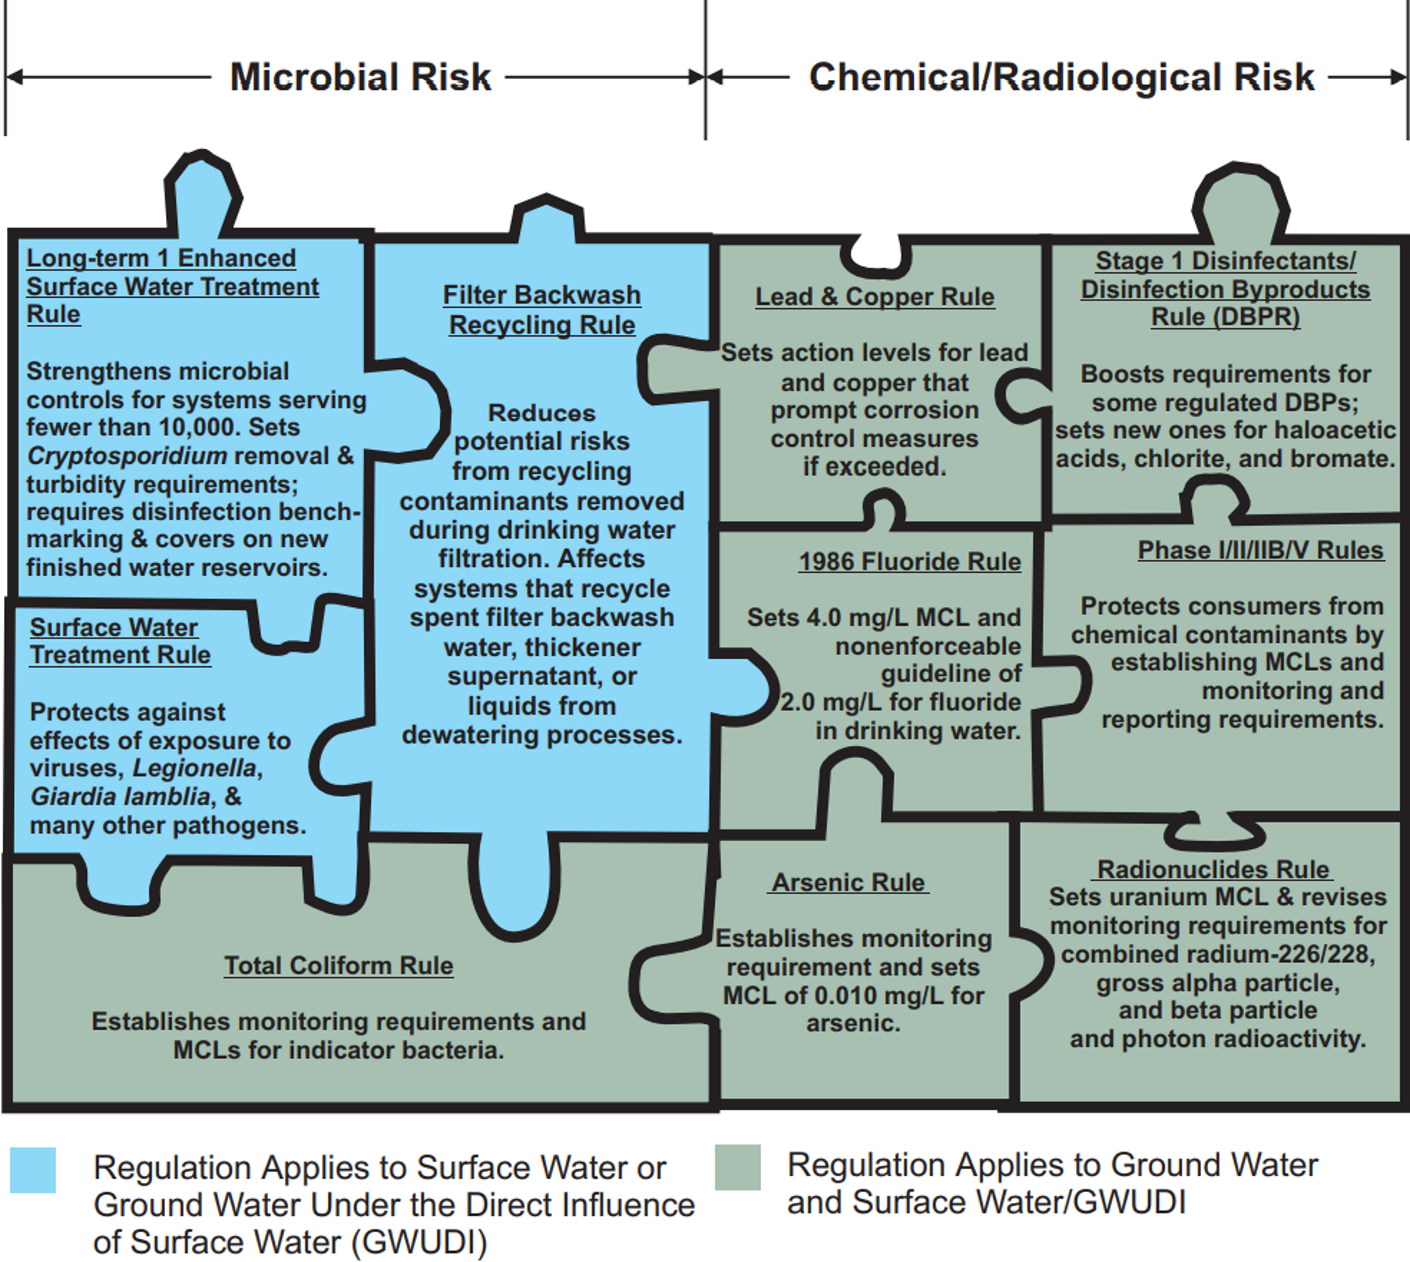
\includegraphics[scale=0.35]{WaterRegulations}
\caption{Summary of water regulations}
\end{center}
\end{figure}

\subsection{Surface Water Treatment Rule}\index{Surface water treatment rule (SWTR)}
\begin{itemize}
\item Adopts a "Multiple Barriers" approach which relies on:
\begin{itemize}
\item \textbf{Pathogen removal} Requires systems to filter unless specific avoidance criteria is met \index{Surface water treatment rule (SWTR)!Pathogen removal}.  
\item \textbf{Pathogen inactivation} \index{Surface water treatment rule (SWTR)!Pathogen inactivation} Requires all systems to disinfect.
\end{itemize}
\item Awards "Credits" for both above. 
\item Requires most water systems to filter and disinfect water from surface water sources or GWUDISW
\item Establishes maximum contaminant level goals (\textbf{MCLGs}) for viruses, bacteria and \textit{Giardia lamblia}
\item Included treatment technique (TT) requirements for filtered and unfiltered systems to protect against adverse health effects of exposure to pathogens


\end{itemize}

\subsection{Interim Enhanced Surface Water Treatment Rule}\index{Interim enhanced surface water treatment rule (IESWTR)}
\begin{itemize}
\item The 1998 Interim Enhanced Surface Water Treatment Rule (\textbf{IESWTR}) increased the level of protection from exposure to Cryptosporidium and other pathogens in drinking water supplies through improvements in filtration at water systems, provided under the original SWTR.
\item IESWTR applies to all public water systems using surface water, or GWUDISW, that serve 10,000 or more persons
\item The SWTR and the Interim ESWTR includes the following general requirements in order to minimize human exposure to microbial contaminants in drinking water:
\end{itemize}

\subsection{Long-Term 1 Enhanced Surface Water Treatment Rule}\index{Long-term 1 enhanced surface water treatment rule (LT1ESWTR)}
\begin{itemize}
\item The Long-Term 1 Enhanced Surface Water Treatment Rule (\textbf{LT1ESWTR}) applies to all public water systems using surface water, or GWUDISW, serving fewer than 10,000  persons
\item The LT1ESWTR builds upon the framework established for systems serving a population of 10,000 or more in the Interim Enhanced Surface Water Treatment Rule (IESWTR). 
\item While there are small differences between the LT1ESWTR and IESWTR, these differences reflect an effort to reduce burden for small systems while still maintaining a comparable level of health protection.
\end{itemize}


\subsection{Long-Term 2 Enhanced Surface Water Treatment Rule}\index{Long-term 2 enhanced surface water treatment rule (LT2ESWTR)}
\begin{itemize}
\item The Long-Term 2 Enhanced Surface Water Treatment Rule (\textbf{LT2ESWTR}) applies to all PWSs that use surface water or GWUDISW
\item Targets additional Cryptosporidium treatment requirements to higher risk systems
\item Requires provisions to reduce risks from uncovered finished water storage facilities
\item Provides provisions to ensure that systems maintain microbial protection as they take steps to reduce the formation of disinfection byproducts
\end{itemize}

\subsection{Requirements under Surface Water Treatment Rules} \index{Surface water treatment rule (SWTR)!Requirements}
\begin{itemize}
\item Utilities are required to achieve at least:
\begin{itemize}
\item 99.9\% removal and/or inactivation of Giardia lamblia cysts (3-log removal)
\item Minimum 99.99\% removal and/or inactivation of viruses (4-log removal)
\item A 2-log removal of Cryptosporidium. 
\end{itemize}

\item Control of Cryptosporidium \index{Control of cyrptosporidium}:
\begin{itemize}
\item The maximum contaminant level goal (MCLG) is set at zero.
\item Filtered systems must physically remove 99\% (2-log) of Cryptosporidium.
\item  Unfiltered systems must update their watershed control programs to  minimize the potential for contamination by Cryptosporidium oocysts
\end{itemize}
\item Removal credit:
\vspace{0.3cm}
\begin{itemize}
\item The level of removal credit given a utility for both Giardia lamblia and viruses is determined by the type of treatment process used. 
\item For a conventional water treatment plant the SWTR provides a 2.5-log removal credit for Giardia lamblia and a 2.0-log removal credit for viruses. 
\item water treatment plants meeting the turbidity performance standard of 0.3 NTU in 95\% of the monthly measurements also get credit for a 2-log reduction in Cryptosporidium.
\end{itemize}
\vspace{0.3cm}
\item Disinfection credit:
\vspace{0.3cm}
\begin{itemize}
\item Disinfection during conventional treatment (assuming all operational criteria and performance standards are met), must achieve 0.5-log inactivation of Giardia lamblia and 2.0-log inactivation of viruses. 
\item As a substitute to actually measuring the inactivation of Giardia lamblia and viruses achieved at a treatment plant, the SWTR established the concept of CT to evaluate inactivation. CT is the product of the concentration of disinfectant remaining at the end of a treatment process (“C” in milligrams per liter) and the contact time in which 10\% of the water passes through the treatment process (“T” or “T10” in minutes). The SWTR provides tables which identify the log removal of both Giardia lamblia and viruses achieved for a calculated CT value based on the type of disinfectant, the water temperature, and pH.
\end{itemize}
\item Turbidity monitoring requirements include:
\begin{itemize}
\item For treatment plants using conventional treatment or direct filtration, a turbidity performance standard for the combined filter effluent (CFE) \index{Combined filter effluent (CFE)} of 1 NTU as a maximum, and 0.3 NTU as a maximum in 95 percent of monthly measurements, based on 4-hour monitoring.
\item Continuous monitoring of individual filter effluent (IFE) \index{Individual filter effluent (IFE)} turbidity in conventional and direct filtration plants and recording of IFE turbidity readings every 15 minutes.
\end{itemize}
\item Reporting and recordkeeping requirements include \index{Surface water treatment rule (SWTR)!Reporting and recordkeeping}:
\begin{itemize}
\item PWSs must report turbidity measurements related to CFE monitoring to the state within 10 days after the end of each month the PWS serves water to the public.

\item PWSs must keep CFE turbidity monitoring records and any other turbidity analyses, with the exception of IFE monitoring records, for at least 5 years. 

\item PWSs must keep records from IFE turbidity monitoring for at least 3 years.
\end{itemize}
\item If a system meets the turbidity performance standard of 0.3 NTU in 95\% of the samples taken each month (never to exceed 1 NTU) than the system gets credit for achieving the 2-log reduction in Cryptosporidium.

\item PWSs using alternative filtration techniques [defined as filtration other than conventional, direct, slow sand, or diatomaceous earth (DE)] must demonstrate to the state the ability to consistently achieve 2-log removal of Cryptosporidium and comply with specific state-established CFE turbidity requirements.


\item The required level of removal/inactivation must occur between the point where the raw water is not longer subject to surface water runoff and the point at which the first customer is served.

\item The disinfectant residual entering the distribution system must not fall below 0.2 mg/L for more than 4 hr during any 24- hr period.

\item A disinfectant residual must be detectable in 95\% of distribution system samples. A heterotrophic plate count (HPC) \index{Heterotrophic plate count} concentration of less than 500 colonies per milliliter can serve as a detectable residual if no residual is measured.

\item Each utility must perform a watershed sanitary survey at least every 5 years.

\end{itemize}
\begin{figure}[H]
\begin{center}
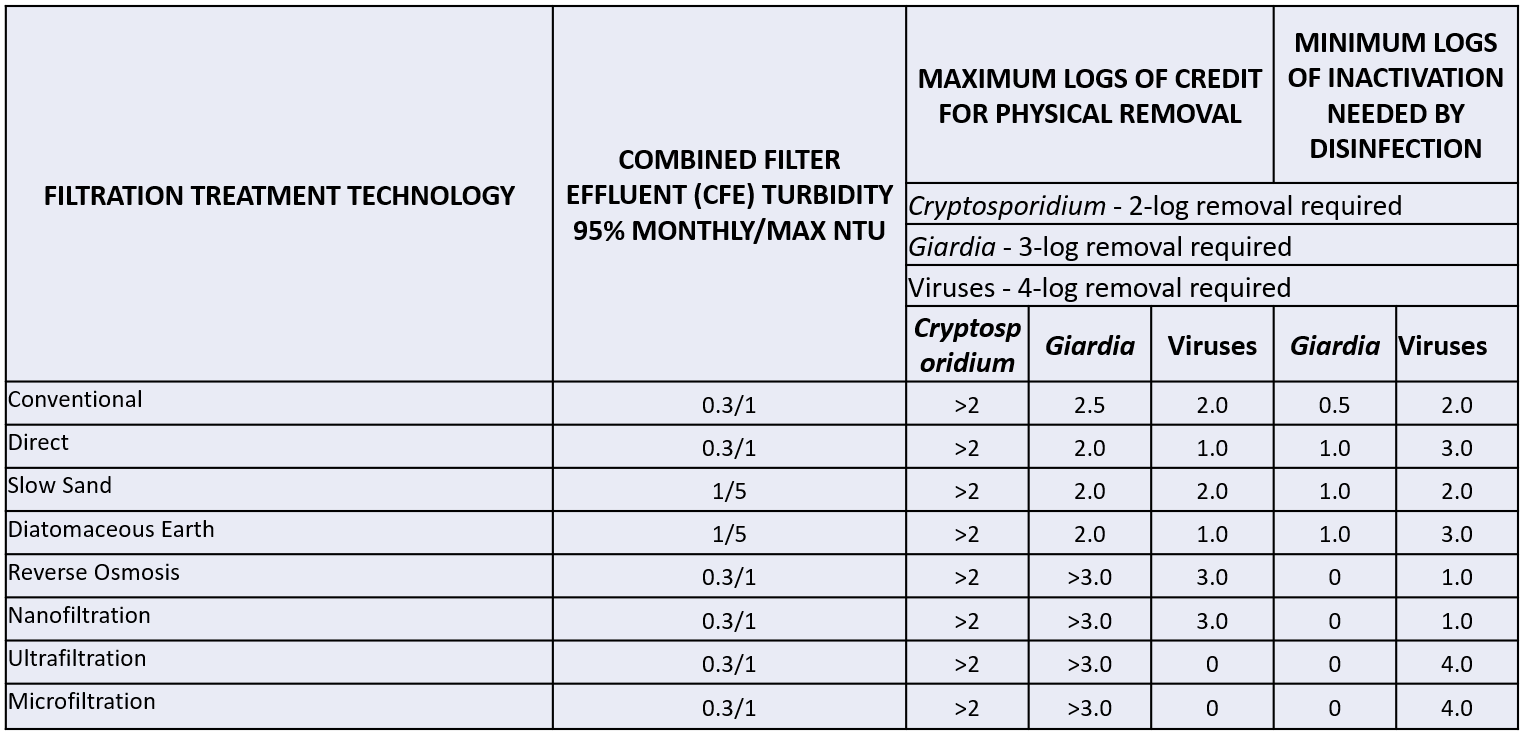
\includegraphics[scale=0.35]{SWTRAutoRemovalCredits}
\caption{SWTR auto removal credits}
\end{center}
\end{figure}


\nopagebreak


\newpage
\thispagestyle{empty}
\begin{landscape}
\begin{table}[h!]
  \centering
\small
\begin{tabular}{|lllll|}
\hline
\rowcolor[HTML]{CBCEFB} 
\multicolumn{2}{|l|}{\cellcolor[HTML]{CBCEFB}TCR/ Nitrate/Nitrite}                                                   & \multicolumn{1}{l|}{\cellcolor[HTML]{CBCEFB}CWS} & \multicolumn{1}{l|}{\cellcolor[HTML]{CBCEFB}NTNCWS} & TNCWS                      \\ \hline
\multicolumn{2}{|l|}{Sanitary Survey}                                                                                & \multicolumn{1}{l|}{Every 3 years}               & \multicolumn{1}{l|}{Every 5 years}                  & Every 5 years              \\ \hline
\multicolumn{2}{|l|}{Total Coliform Bacteria1}                                                                       & \multicolumn{1}{l|}{Monthly}                     & \multicolumn{1}{l|}{Monthly}                        & Monthly                    \\ \hline
\multicolumn{2}{|l|}{Nitrate (NO$_3$)}                                                                                  & \multicolumn{1}{l|}{Quarterly$^2$}                  & \multicolumn{1}{l|}{Quarterly$^2$}                     & Annually                   \\ \hline
\multicolumn{2}{|l|}{Nitrite (NO$_2$)}                                                                                  & \multicolumn{1}{l|}{1 sample record}             & \multicolumn{1}{l|}{1 sample record}                & 1 sample record            \\ \hline
\rowcolor[HTML]{CBCEFB} 
\multicolumn{2}{|l|}{\cellcolor[HTML]{CBCEFB}Reporting}                                                              & \multicolumn{1}{l|}{\cellcolor[HTML]{CBCEFB}CWS} & \multicolumn{1}{l|}{\cellcolor[HTML]{CBCEFB}NTNCWS} & TNCWS                      \\ \hline
\multicolumn{2}{|l|}{}                                                                                               & \multicolumn{1}{l|}{Continuous or grab samples}  & \multicolumn{1}{l|}{Continuous or grab samples}     & Continuous or grab samples \\ \hline
\multicolumn{2}{|l|}{Turbidity}                                                                                      & \multicolumn{3}{l|}{(Frequency determined by population and   filtration type.)}                                                    \\ \hline
\multicolumn{2}{|l|}{Fluoride – if added}                                                                            & \multicolumn{1}{l|}{Daily}                       & \multicolumn{1}{l|}{Daily}                          &                            \\ \hline
\multicolumn{2}{|l|}{}                                                                                               & \multicolumn{1}{l|}{Continuous or grab samples}  & \multicolumn{1}{l|}{Continuous or grab samples}     & Continuous or grab samples \\ \cline{3-5} 
\multicolumn{2}{|l|}{\multirow{-2}{*}{Entry Point Chlorine – if chlorine is added}}                                  & \multicolumn{3}{l|}{(Pop determines how many times a   day chlorine is measured.)}                                                  \\ \hline
\multicolumn{2}{|l|}{Distribution System Chlorine3}                                                                  & \multicolumn{1}{l|}{Monthly}                     & \multicolumn{1}{l|}{Monthly}                        & Monthly                    \\ \hline
\multicolumn{2}{|l|}{Consumer Confidence Report}                                                                     & \multicolumn{1}{l|}{Annually}                    & \multicolumn{1}{l|}{Annually}                       &                            \\ \hline
\rowcolor[HTML]{CBCEFB} 
\multicolumn{2}{|l|}{\cellcolor[HTML]{CBCEFB}Disinfection/Disinfectant Byproducts}                                   & \multicolumn{1}{|l|}{\cellcolor[HTML]{CBCEFB}CWS} & \multicolumn{1}{|l|}{\cellcolor[HTML]{CBCEFB}NTNCWS} & TNCWS                      \\ \hline
\multicolumn{1}{|l|}{}                                                      & \multicolumn{1}{l|}{Pop \textless 500} & \multicolumn{1}{l|}{Annually}                    & \multicolumn{1}{l|}{Annually}                       & Annually                   \\ \cline{2-5} 
\multicolumn{1}{|l|}{}                                                      & \multicolumn{1}{l|}{Pop 500 -   9,999} & \multicolumn{1}{l|}{Quarterly}                   & \multicolumn{1}{l|}{Quarterly}                      & Quarterly                  \\ \cline{2-5} 
\multicolumn{1}{|l|}{\multirow{-3}{*}{Total   Trihalomethanes (TTHM/HAA5)}} & \multicolumn{1}{l|}{Pop 10,000}        & \multicolumn{1}{l|}{Quarterly}                   & \multicolumn{1}{l|}{Quarterly}                      & Quarterly                  \\ \hline
\multicolumn{2}{|l|}{TOC and Alkalinity}                                                                             & \multicolumn{1}{l|}{Monthly2}                    & \multicolumn{1}{l|}{Monthly2}                       &                            \\ \hline
\multicolumn{2}{|l|}{Bromate (Ozone plants only)}                                                                    & \multicolumn{1}{l|}{Monthly}                     & \multicolumn{1}{l|}{Monthly}                        &                            \\ \hline
\rowcolor[HTML]{CBCEFB} 
\multicolumn{2}{|l|}{\cellcolor[HTML]{CBCEFB}Inorganic Chemicals}                                                    & \multicolumn{1}{l|}{\cellcolor[HTML]{CBCEFB}CWS} & \multicolumn{1}{l|}{\cellcolor[HTML]{CBCEFB}NTNCWS} & TNCWS                      \\ \hline
\multicolumn{2}{|l|}{All Primary}                                                                                    & \multicolumn{1}{l|}{Annually}                    & \multicolumn{1}{l|}{Annually}                       &                            \\ \hline
\multicolumn{2}{|l|}{Arsenic}                                                                                        & \multicolumn{1}{l|}{Annually}                    & \multicolumn{1}{l|}{Annually}                       &                            \\ \hline
\multicolumn{2}{|l|}{Asbestos}                                                                                       & \multicolumn{1}{l|}{Once per period}             & \multicolumn{1}{l|}{Once per period}                &                            \\ \hline
\multicolumn{2}{|l|}{Lead and Copper1}                                                                               & \multicolumn{1}{l|}{Every 6 months$^2$}             & \multicolumn{1}{l|}{Every 6 months$^2$}                &                            \\ \hline
\rowcolor[HTML]{CBCEFB} 
\multicolumn{2}{|l|}{\cellcolor[HTML]{CBCEFB}Organic Chemicals}                                                      & \multicolumn{1}{l|}{\cellcolor[HTML]{CBCEFB}CWS} & \multicolumn{1}{l|}{\cellcolor[HTML]{CBCEFB}NTNCWS} & TNCWS                      \\ \hline
\multicolumn{2}{|l|}{Pesticides (SOCs) and Other Organics}                                                           & \multicolumn{1}{l|}{Quarterly$^2$}                  & \multicolumn{1}{l|}{Quarterly$^2$}                     &                            \\ \hline
\multicolumn{2}{|l|}{}                                                                                               & \multicolumn{1}{l|}{Quarterly}                   & \multicolumn{1}{l|}{Quarterly}                      &                            \\ \cline{3-5} 
\multicolumn{2}{|l|}{\multirow{-2}{*}{Volatile Organic Chemicals (VOCs)}}                                            & \multicolumn{1}{l|}{Annually}                    & \multicolumn{1}{l|}{Annually}                       &                            \\ \hline
\rowcolor[HTML]{CBCEFB} 
\multicolumn{2}{|l|}{\cellcolor[HTML]{CBCEFB}Radionuclides}                                                          & \multicolumn{1}{l|}{\cellcolor[HTML]{CBCEFB}CWS} & \multicolumn{1}{l|}{\cellcolor[HTML]{CBCEFB}NTNCWS} & TNCWS                      \\ \hline
\multicolumn{2}{|l|}{Gross Alpha Radioactivity}                                                                      & \multicolumn{1}{l|}{Quarterly}                   & \multicolumn{1}{l|}{}                               &                            \\ \hline
\multicolumn{2}{|l|}{Radium 226, Radium 228, Uranium}                                                                & \multicolumn{1}{l|}{Quarterly}                   & \multicolumn{1}{l|}{}                               &                            \\ \hline

\multicolumn{5}{|l|}{\begin{tabular}[c]{@{}l@{}}$^1$ Number of samples is based on   population.\\     $^2$   May be   reduced if certain criteria are met.\\      $^3$   Distribution point chlorine   test is required at the same time and location as total coliform samples are   collected\\Cycle - 3 years\\ Period – 9 years\end{tabular}}

\\ \hline
\end{tabular}
%
%
%
%
%
%
%
%
%
%\multicolumn{5}{|l|}{1 Number of samples is based   on population. 2 May be   reduced if certain criteria are met.}                                                                                                                                        \\ \hline
%\multicolumn{5}{|l|}{3 Distribution point chlorine   test is required at the same time and location as total coliform samples are   collected.}                                                                                                            \\ \hline
%\multicolumn{5}{|l|}{Cycle – 3 years; Period – 9 years}                                                                                                                                                                                                    \\ \hline
%\end{tabular}
\caption{Sampling and testing schedules for surface water and GUDISW}
%\textit{(Source:Introduction to Small Water Systems - Alaska DEC)}

\end{table}
\end{landscape}

\section{Total Coliform Rule}\index{Total coliform rule (TCR)}
\begin{itemize}
\item The 1989 Total Coliform Rule (\textbf{TCR})promotes surveillance of distribution system water quality targeting fecal matter and/or pathogens.
\item Rule requires collection of monthly samples that are representative of water throughout the distribution system as identified in its approved Sample Siting Plan.
\item For systems serving >1,000 people, number of monthly samples that need to be collected is based upon the population served.  
\item The presence of total coliforms is a warning sign that the system is vulnerable to contamination. It does not necessarily mean that the system is contaminated.
\item If sample is total coliform (TC) positive:
\begin{enumerate}[A.]
\item Conduct follow up testing:
\begin{enumerate}[1.]
\item In the same sample, determine fecal coliform (FC) or E. Coli (EC).
\item Collect a second sample within 24 hours, and reanaylze TC and FC/EC. 
\end{enumerate}
\item The system is not in compliance if:
\begin{enumerate}[i.]
\item The analysis and reanalysis of a given sampling location are TC positive (TC[+]) both times and FC[/EC+] at least one of these times. \textbf{OR}
\item More than 5 percent of all monthly samples for a 12-month period are TC[+].
\end{enumerate}
\end{enumerate}

\end{itemize}

\begin{figure}[]
\begin{center}
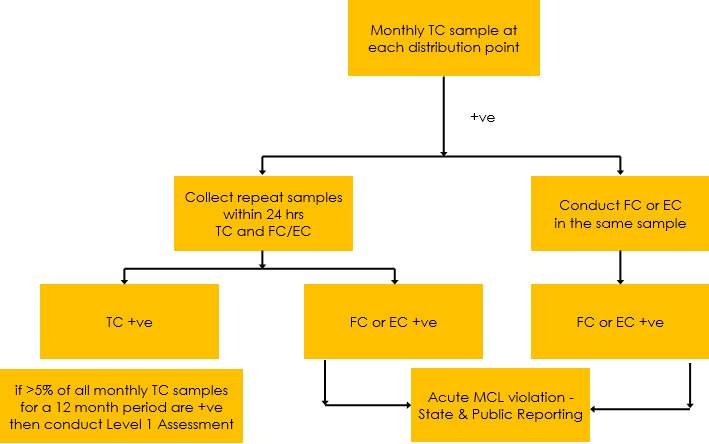
\includegraphics[scale=0.65]{TCRSummary}
\caption{Summary of Total Coliform Rule requirements}
\end{center}
\end{figure}




\subsection{Revised Total Coliform Rule}\index{Revised total coliform rule (RTCR)}
\begin{itemize}
\item The 2013 Revised Total Coliform Rule (\textbf{rTCR})revises the 1989 Total Coliform Rule (\textbf{TCR}) and is applicable to all PSWs. 
\item Establishes a \textbf{zero} MCL and MCLG for EC and eliminated MCLG and MCL for TC.  EC being a more specific indicator of fecal contamination and potentially harmful pathogens than
TC and also many of the organisms detected by total coliform methods are not of fecal origin and do not have any direct public health implication. 
\item The revised rule changes total coliform detection from a MCL to a Treatment Technique
Trigger, requiring the PWS to perform a system review and fix any potential breaches in
the microbiological barriers. Detection of E. coli during sampling indicates the
exceedance of the MCL. These detections also trigger an inspection and correction of any
sanitary defects found. The rTCR also increases monitoring for many systems experiencing compliance issues or that do not have a microbiologically protected source.
\item Requirements for monitoring TC and EC according to a sample siting plan and schedule specific to the PWS.
\item Requires sampling site representative of the entire distribution system.
\item Eliminated TCR's public notification requirements based only on the presence of TC and instead requires public notification when:
\begin{enumerate}
\item When an an EC MCL violation occurs \textbf{OR}
\item When a PWS fails to conduct the required assessment and corrective action.
\end{enumerate}
\item Uses vulnerable PWS to initiate a "find and fix" approach to address fecal contamination that could enter the distribution system.
\item rTCR requires PWS to perform assessments to identify sanitary defects - that could provide a pathway of entry for microbial contamination, or those that indicate failure (existing or potential) of protective barriers against microbial contamination, and subsequently take action to correct them.
\item There are two levels of assessments based on the severity or frequency of the problem:
\begin{enumerate}
\item A Level 1 assessment is required if:
\begin{itemize}
\item For systems taking 40 or more samples per month, the utility exceeds 5.0 percent total coliform-positive samples for the month; or
\item For systems taking fewer than 40 samples per month, the utility has two or more total coliform-positive samples in the same month; or
\item The Utility fails to take every required repeat sample after any single routine total coliform-positive sample.
\end{itemize}

\item Level 2 which is an in-depth examination of the distribution system, water sources, treatment facilities, storage facilities and relevant operational practices at a public water system (PWS) conducted by an assessor - state or state-approved entity. Level 2 assessment is triggered by an E.Coli MCL violation or a second Level 1 assessment in a 12-month period or in two consecutive years.
\item When sanitary defects are identified during a Level 1 or Level 2 Assessment, they should be corrected as soon as possible to protect public health.
\end{enumerate}

\item A public water system will receive a Treatment Technique violation when any of the following occur:
\begin{itemize}
\item Failure to conduct a Level 1 or Level 2 Assessment within 30 days of a trigger.
\item Failure to correct all sanitary defects from a Level 1 or Level 2 Assessment within
30 days of a trigger or in accordance with the state-approved time frame.
\item Failure of a seasonal system to complete state-approved start-up procedures prior to serving water to the public.
\end{itemize}
\end{itemize}

\subsection{Filter Backwash Recycle Rule}\index{Filter backwash recycle rule}
\begin{itemize}
\item Filter Backwash Recycle Rule (\textbf{FBRR})applies to all public water systems using conventional or direct filtration to treat surface water, or GWUDISW, regardless of size
\item Requires PWSs to review their backwash water recycling practices to ensure that they do not compromise microbial control
\item Requires recycled filter backwash water to go through all processes of a system’s conventional or direct filtration treatment. 
\end{itemize}

\section{Groundwater rules}\index{Groundwater rules}
\begin{itemize}
\item The Federal Groundwater Rules (\textbf{GWR}) rule applies to public water systems that use groundwater as a source of drinking water.
\item Goal of the GWR is increased protection against microbial pathogens. 
\item groundwater systems that are at risk of fecal contamination must take corrective action. Corrective action reduces potential illness from exposure to microbial pathogens. The 
\item The GWR relies on four major components:
\begin{enumerate}
\item Routine sanitary surveys of systems that require the evaluation of critical elements of a public water system and the identification of significant deficiencies (e.g., a well located near a leaking septic system);
\item Triggered source water monitoring for a system that (not treating drinking water to remove 99.99 percent (4-log) of viruses) identifies a positive sample during regular Total Coliform monitoring or assessment monitoring (at the option of the state) targeted at high-risk systems
\item Corrective action is required for any system with a significant deficiency or source water fecal contamination; and
\item Compliance monitoring to ensure that treatment technology installed to treat drinking water reliably achieves 99.99 percent (4-log) inactivation or removal of viruses.
\end{enumerate}
\item In California, the Sustainable Groundwater Management Act (\textbf{SGMA})sets a timeline to identify responsible local agencies – which will work as a team – the means to reverse overdrafted conditions in certain areas and to ensure the 127 “high and medium priority” groundwater basins or sub-basins not in overdraft reach sustainability by 2040.
\end{itemize}

\newpage
\thispagestyle{empty}
\begin{landscape}
\begin{table}[h!]
  \centering
\small
\begin{tabular}{|l|l|l|l|l|}
\hline
\rowcolor[HTML]{CBCEFB} 
\multicolumn{2}{|l|}{\cellcolor[HTML]{CBCEFB}\textbf{TCR/ Nitrate/Nitrite}}                                             & \multicolumn{1}{l|}{\cellcolor[HTML]{CBCEFB}\textbf{CWS}}             & \multicolumn{1}{l|}{\cellcolor[HTML]{CBCEFB}\textbf{NTNCWS}}             & \multicolumn{1}{l|}{\cellcolor[HTML]{CBCEFB}\textbf{TNCWS}}             \\ \hline
\multicolumn{2}{|l|}{Sanitary Survey}                                                                                   & Every 5 years                                                        & Every 5 years                                                           & Every 5 years                                                          \\
\multicolumn{2}{|l|}{Total Coliform Bacteria$^1$}                                                                          & Every month                                                          & Every month                                                             & Every quarter                                                          \\
\multicolumn{2}{|l|}{Nitrate (NO3)}                                                                                     & Annually                                                             & Annually                                                                & Annually                                                               \\
\multicolumn{2}{|l|}{Nitrite (NO2)}                                                                                     & 1 sample record                                                      & 1 sample record                                                         & 1 sample record                                                        \\ \hline
\rowcolor[HTML]{CBCEFB} 
\multicolumn{2}{|l|}{\cellcolor[HTML]{CBCEFB}\textbf{Reporting}}                                                        & \multicolumn{1}{l|}{\cellcolor[HTML]{CBCEFB}\textbf{CWS}}             & \multicolumn{1}{l|}{\cellcolor[HTML]{CBCEFB}\textbf{NTNCWS}}             & \multicolumn{1}{l|}{\cellcolor[HTML]{CBCEFB}\textbf{TNCWS}}             \\ \hline
\multicolumn{2}{|l|}{Fluoride – if added}                                                                               & Daily                                                                & Daily                                                                   & Daily                                                                  \\
\multicolumn{2}{|l|}{}                                                                                                  & Continuous or grab samples                                           & Continuous or grab samples                                              & Continuous or grab samples                                             \\
\multicolumn{2}{|l|}{\multirow{-2}{*}{Entry Point Chlorine – if chlorine is added}}                                 & \multicolumn{3}{|l|}{(Pop determines how many times   a day chlorine is measured.)}                                                                                                                                       \\
\multicolumn{2}{|l|}{Distribution Chlorine$^2$ – if chlorine is added}                                                   & Monthly                                                              & Monthly                                                                 &                                                                        \\
\multicolumn{2}{|l|}{Consumer Confidence Report}                                                                        & Annually                                                             &                                                                         &                                                                        \\ \hline
\rowcolor[HTML]{CBCEFB} 
\multicolumn{2}{|l|}{\cellcolor[HTML]{CBCEFB}\textbf{Disinfection/Disinfectant Byproducts}}                         & \multicolumn{1}{l|}{\cellcolor[HTML]{CBCEFB}\textbf{CWS}}             & \multicolumn{1}{l|}{\cellcolor[HTML]{CBCEFB}\textbf{NTNCWS}}             & \multicolumn{1}{l|}{\cellcolor[HTML]{CBCEFB}\textbf{TNCWS}}             \\
                                                                         & Pop \textless 500 – 9,999                  & Annually                                                             & Annually                                                                &                                                                        \\
\multirow{-2}{*}{Total Trihalomethanes$^1$ (TTHM/HAA5)}                   & Pop $\geq$ 10,000                                & Quarterly                                                            & Quarterly                                                               &                                                                        \\ \hline
\multicolumn{2}{|l|}{Bromate (Ozone plants only)}                                                                       & Monthly                                                              & Monthly                                                                 &                                                                        \\ \hline
\rowcolor[HTML]{CBCEFB} 
\multicolumn{2}{|l|}{\cellcolor[HTML]{CBCEFB}Inorganic Chemicals}                                                       & \multicolumn{1}{l|}{\cellcolor[HTML]{CBCEFB}CWS}                      & \multicolumn{1}{l|}{\cellcolor[HTML]{CBCEFB}NTNCWS}                      & \multicolumn{1}{l|}{\cellcolor[HTML]{CBCEFB}TNCWS}                      \\ \hline
\multicolumn{2}{|l|}{All Primary}                                                                                       & Once per period                                                      & Once per period                                                         &                                                                        \\
\multicolumn{2}{|l|}{Arsenic}                                                                                           & Once per period                                                      & Once per period                                                         &                                                                        \\
\multicolumn{2}{|l|}{Asbestos}                                                                                          & Once per cycle                                                       & Once per cycle                                                          &                                                                        \\
\multicolumn{2}{|l|}{Lead and Copper$^1$}                                                                                  & Every 6 months$^3$                                                      & Every 6 months$^3                                                        $ &                                                                        \\ \hline
\rowcolor[HTML]{CBCEFB} 
\multicolumn{2}{|l|}{\cellcolor[HTML]{CBCEFB}\textbf{Organic Chemicals}}                                                & \multicolumn{1}{l|}{\cellcolor[HTML]{CBCEFB}\textbf{CWS}}             & \multicolumn{1}{l|}{\cellcolor[HTML]{CBCEFB}\textbf{NTNCWS}}             & \multicolumn{1}{l|}{\cellcolor[HTML]{CBCEFB}\textbf{TNCWS}}             \\ \hline
\multicolumn{2}{|l|}{Pesticides (SOCs) and Other   Organics}                                                            & Every quarter3                                                       & Every quarter3                                                          &                                                                        \\
\multicolumn{2}{|l|}{}                                                                                                  & Every quarter                                                        & Every quarter                                                           &                                                                        \\
\multicolumn{2}{|l|}{\multirow{-2}{*}{Volatile Organic Chemicals   (VOCs)}}                                             & Annually                                                             & Annually                                                                &                                                                        \\ \hline
\rowcolor[HTML]{CBCEFB} 
\multicolumn{2}{|l|}{\cellcolor[HTML]{CBCEFB}\textbf{Radionuclides}}                                                    & \multicolumn{1}{c}{\cellcolor[HTML]{CBCEFB}\textbf{CWS}}             & \multicolumn{1}{c}{\cellcolor[HTML]{CBCEFB}\textbf{NTNCWS}}             & \multicolumn{1}{c}{\cellcolor[HTML]{CBCEFB}\textbf{TNCWS}}             \\
\multicolumn{2}{|l|}{Gross Alpha Radioactivity}                                                                         & Every quarter                                                        &                                                                         &                                                                        \\
\multicolumn{2}{|l|}{Radium 226, Radium 228, Uranium}                                                                   & Every quarter                                                        &                                                                         &                                                                       
\\ \hline
\multicolumn{5}{|l|}{\begin{tabular}[c]{@{}l@{}}$^1$ Number of samples is based on   population.\\     $^2$   Distribution   point chlorine test is required at the same time and location as total   coliform samples are collected.\\      $^3$   May   be reduced if certain criteria are met.\\      Cycle – 3 years\\      Period – 9 years\end{tabular}}\\
\hline
\end{tabular}
\caption{Sampling and testing schedules for groundwater}
\end{table}
\end{landscape}

\section{Microbial and disinfection byproducts rules}\index{Microbial and disinfection byproducts rules}
\begin{itemize}
\item The Microbial and Disinfection Byproducts Rules (\textbf{MDBPs}) include Stage 1 and Stage 2 Disinfectants and Disinfection Byproducts Rules (\textbf{DBPRs}) 
\item As disinfectants can react with naturally-occurring materials in the water to form byproducts including:
\begin{itemize}
\item Trihalomethanes (THM),
\item Haloacetic acids (HAA),
\item Chlorite, and
\item Bromate.
\end{itemize}
\item The Stage 1 and Stage 2 DBPRs are intended to minimize the public
health risk from DBPs and disinfectants that are used to control pathogens.
\item Under these rules, EPA established:
\begin{itemize}
\item Maximum residual disinfectant levels (MRDLs) \index{Maximum residual disinfectant levels (MRDLs)}for chlorine, chloramines and chlorine dioxide, and
\item  MCLs for DBPs - chlorite, bromate, TTHM and HAA5.
\end{itemize}
\item These Rules apply to all Community Water Systems (\textbf{CWS}) and Non-Transient Non-Community Water Systems (\textbf{NTNCWS}) that add/deliver a primary or residual disinfectant, and TNCWs that use chlorine dioxide. 
\item This Rule does not apply to water systems that use ultraviolet (UV) light.
\item The maximum residual disinfectant levels (\textbf{MRDLs}), and maximum residual disinfectant level goals (\textbf{MRDLGs}) for the three chemical disinfectants are listed in Table \ref{table:DisinfectantMRDLs} \index{Disinfectant MRDLs}.
\item The MCLs for DBPs are listed in Table \ref{table:DBPMCL}.
\begin{table}[]
\begin{center}
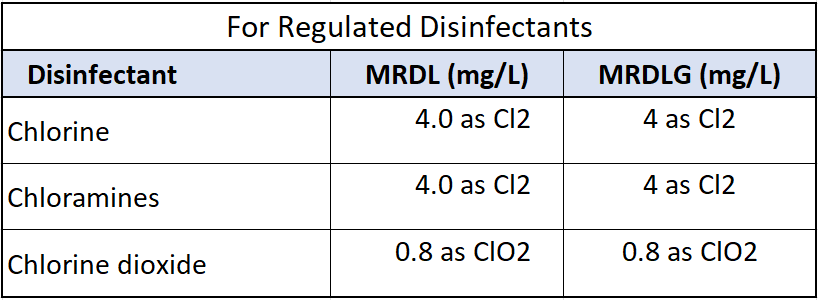
\includegraphics[scale=0.5]{DinfectantMRDLS}
\caption{Disinfectant MRDLs}
\label{table:DisinfectantMRDLs}
\end{center}
\end{table}
\begin{table}[]
\begin{center}
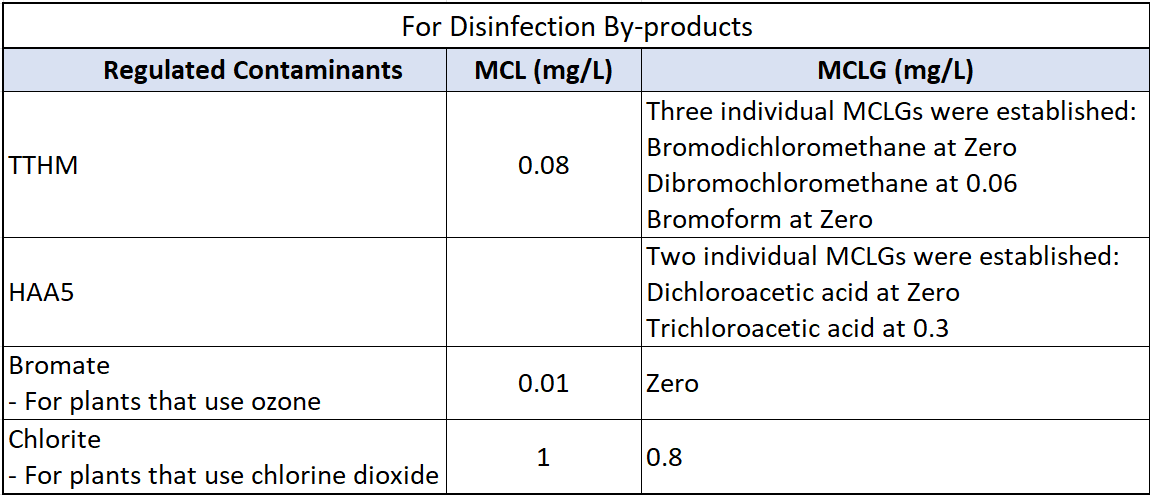
\includegraphics[scale=0.5]{DBPMCLS}
\caption{Disinfectant by-products MCLs}
\label{table:DBPMCL}
\end{center}
\end{table}
\item Compliance is based on a running annual average (RAA) calculated quarterly, locational running annual average (LRAA) calculated quarterly, a single sample result or an average of a selected number of samples, depending on which disinfectant or DBP is being monitored.
\item If the creation of these by-products causes the system to exceed the MCL for Total TTHMs (0.1 mg/l or 100 ppb), the system will be required to change to a different means of disinfection. 
\item Total chlorine residuals are also limited to a maximum of 4.0 mg/l. 
\item The D-DBP rule currently only applies to systems serving a population over 10,000.
\end{itemize}
\section{Other drinking water rules}
\subsection{Lead and Copper Rule}\index{Lead and copper rule}
\begin{itemize}
\item The objective of the 1991 Lead and Copper Rule (\textbf{LCR}) is to control corrosiveness of the finished water in drinking water distribution systems to limit the amount of lead (Pb) and copper (Cu) that may be leached from certain metal pipes and fittings in the distribution system.
\item Applies to all community water systems (CWSs) and non-transient non-community water systems (NTNCWSs)that use groundwater as a source of drinking water.
\item Establishes action level (AL) of 0.015 mg/L for Pb and 1.3 mg/L for Cu based on 90th percentile level of tap water samples.  The rule also establishes an MCLG of \textbf{zero} for lead.
\item The lead action level is a measure of the effectiveness of the corrosion control treatment
in water systems. The action level is not a standard for establishing a safe level of lead in a
home. 
\item Number of samples is based on system size - population served and Systems must conduct monitoring every 6 months unless they qualify for reduced monitoring. 
\item Utilities are required to identify sampling locations and determining initial tap water Pb and Cu levels and also monitor other water quality parameters (WQPs) at these locations to monitor and evaluate the corrosion control characteristics of supplied water.
\item Each utility must complete a survey and evaluate materials that comprise their distribution system, in addition to using other available information, to target homes that are at high risk for Pb/Cu contamination.
\item An AL exceedance is not a violation but can trigger other requirements that include water quality parameter (WQP) monitoring, corrosion control treatment (CCT), source water monitoring/treatment, public education, and lead service line replacement (LSLR).
\item Pb, Cu, and WQPs are initially collected at 6-month intervals.  This frequency can be reduced if action levels are not exceeded and optimal water treatment is maintained.
\item Systems that are in noncompliance and are performing additional corrosion-control activities must continue to monitor at six-month intervals, plus they must collect WQPs from distribution system entry points every two weeks.
\begin{table}[H]
\begin{center}
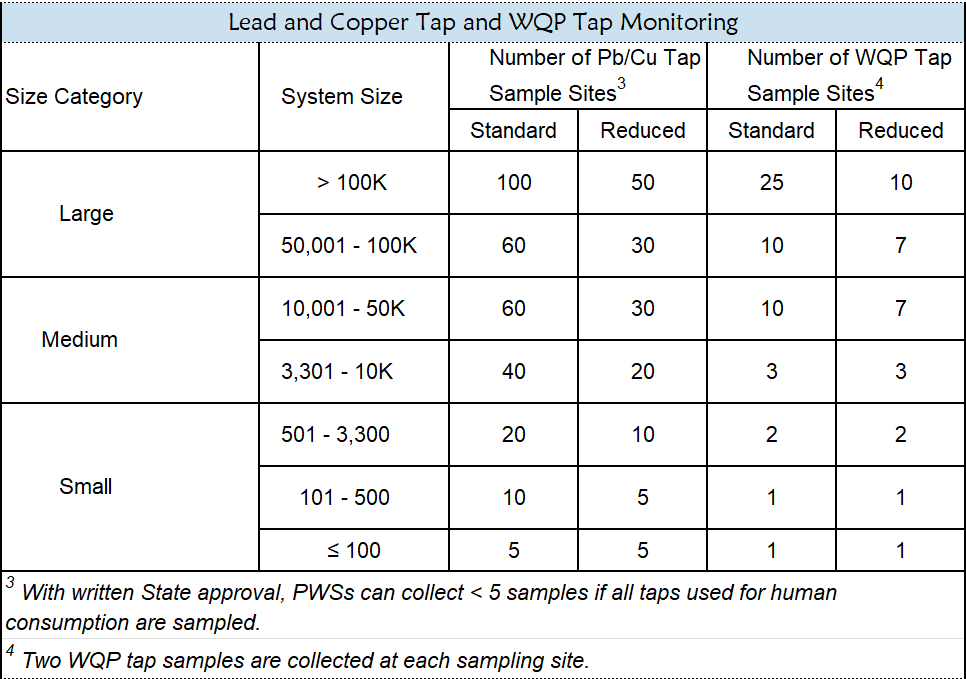
\includegraphics[scale=0.5]{LCRMonitoring}
\caption{Lead and copper tap and WQP tap monitoring}
\end{center}
\end{table}
\end{itemize}

\subsection{Radionuclides Rule}\index{Radionuclides Rule}
\begin{itemize}
\item The 2000 Radionuclide Rule regulates radionuclides in drinking water to protect public health. 
\item Radionuclides are radioactive elements which mostly enters the drinking water source from natural sources.
\item Radiation from radionuclide is known to cause cancer.
\item Radionuclide Rule applies only to Community Water Systems.
\item The rule extablishes the MCLs for radionuclides.
\newpage
\begin{figure}[H]
\begin{center}
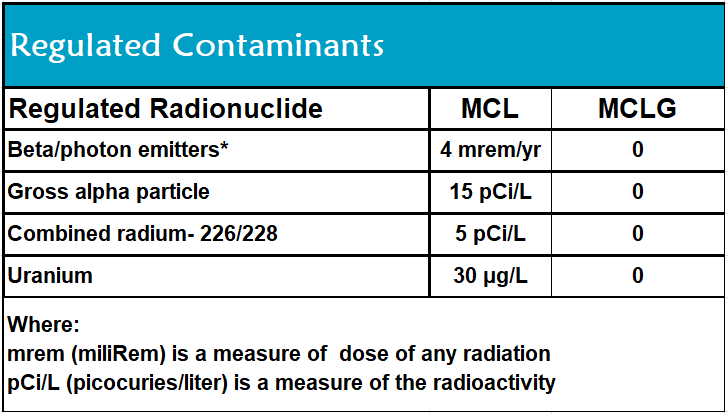
\includegraphics[scale=0.5]{RadionuclideMCL}
\caption{Radionuclide MCLs}
\end{center}
\end{figure}

\item Systems violating the MCL for one of the radionuclide, are required to work with the state to identify and implement options which may include finding a better source of water or blending.
\end{itemize}

\subsection{Arsenic Rule}\index{Arsenic Rule}
\begin{itemize}
\item Arsenic is released to the environment from a variety of natural and anthropogenic
sources. 
\begin{itemize}
\item In the environment, arsenic occurs in rocks, soil, water, air, and in biota.
\item Anthropogenic sources of arsenic relate to its use as wood preservative and in agriculture, livestock, and general industries. 
\end{itemize}
\item There is evidence that associates chronic arsenic ingestion at low concentrations with
increased risk of skin cancer, and that arsenic may cause cancers of the lung, liver, bladder,
kidney, and colon.
\item This rule establishes an Arsenic MCL of 10 ppb.

\end{itemize}
\subsection{Vulnerability assessment} \index{Vulnerability assessment}
\begin{itemize}
\item Under the Public Health Security and Bioterrorism Preparedness and Response Act of 2002,  community water systems that serve populations of greater than 3,300 persons are required to conduct vulnerability assessments.

\item Vulnerability assessments help water systems evaluate susceptibility to potential threats
and identify corrective actions that can reduce or mitigate the risk of serious consequences from
malevolent acts and natural hazards. 
. 

\item Such an assessment for a water system takes into account the vulnerability of the water supply (both ground and surface water), transmission, treatment, and distribution systems. It also considers risks posed to the surrounding community related to attacks on the water system. 

\item An effective vulnerability assessment serves as a guide to the water utility by providing a prioritized plan for security upgrades, modifications of operational procedures, and/or policy changes to mitigate the risks and vulnerabilities to the utility’s critical assets. 

\item Water systems should review their vulnerability assessments periodically to account for changing threats or additions to the system to ensure that security objectives are being met. 


\item Preferably, a vulnerability assessment is "performance-based,” meaning that it evaluates the risk to the water system based on the effectiveness (performance) of existing and planned measures to counteract adversarial actions.
\end{itemize}

\subsection{Public Notification Rule}\index{Public Notification Rule}
\begin{itemize}
\item Public Notification (\textbf{PN}) Rule requires PWS to notify their customers when:
\begin{itemize}
\item If they violate EPA or state drinking water regulations (including monitoring requirements), or 
\item If they provide drinking water that may pose a risk to consumer’s health.
Water systems test regularly for approximately 90 contaminants. The monitoring ensures identification of regulated contaminants at levels which may pose a risk to human health.
\end{itemize}
\item Public notice requirements are divided into three tiers to take into account the seriousness of the violation or situation and of any potential adverse health effects that may be involved.\\
\vspace{0.2cm}
\textbf{Tier 1:} \index{Public Notification Rule!Tiers 1, 2 and 3}\\
\begin{itemize}
\item A Tier 1 notice is required for violations and situations with significant potential to have serious adverse effects on human health as a result of short-term exposure, including but not limited to the following:.
\begin{itemize}
\item Distribution system sample violation when fecal coliform or E. coli are present
\item Failure to test for fecal coliform or E. coli after initial total coliform distribution system sample tests positive.
\item Nitrate, nitrite, or total nitrate and nitrite MCL  violation; failure to take confirmation	sample.
\item Exceedance of maximum allowable turbidity level, if elevated to a Tier 1 notice by primacy agency.
\item Waterborne disease outbreak or other waterborne emergency.
\item Detection of \textit{E. coli}, \textit{enterococci}, or \textit{coliphage} in a groundwater source sample.
\end{itemize}
\item Tier 1 PN is required to be issued as soon as practical but no later than 24 hours after the PWS learns of the violation or situation.
\item The form and manner of Tier 1 PN used must reach all persons served.
\item One or more of the following forms of delivery must be used:
\begin{itemize}
\item Appropriate broadcast media such as radio and television.
\item Posting of the notice in conspicuous locations throughout the area served by the water system;
\item Hand delivery of the notice to persons served by the water system.
\end{itemize}
\item Water suppliers must repeat tier 1 notices at least once every three months or more frequently at the discretion of the Authority, as long as the violation or situation persists.
\end{itemize}
\end{itemize}
\vspace{0.2cm}
\textbf{Tier 2:}
\begin{itemize}
\item Tier 2 PN is required for all violations and situations with potential to have serious adverse effects on human health, including but not limited to:
\begin{itemize}
\item All MCL, MRDL, and treatment technique violations, except where Tier 1 notice is required.
\item Monitoring violations, if elevated to Tier 2 notice by primacy agency.
\item For	ground	water	systems	providing	4-log	treatment	and	conducting	GWR	compliance monitoring, failure to maintain required treatment for more than 4 hours.
\end{itemize}
\item Tier 2 PN is required to be issued as soon as practical, but no later than 30 days after learning of the violation or situation.
\item Community water systems may provide notice by mail or other direct delivery to each customer receiving a bill and to other service connections to which water is delivered by the public water system.
\end{itemize}

\vspace{0.2cm}
\textbf{Tier 3:}\\
\begin{itemize}
\item Tier 3 PN is required for other violations or situations not included in Tier 1 and 2,including but not limited to the ones listed below.
\begin{itemize}
\item All monitoring or testing procedure violations, unless primacy agency elevates to Tier 2, including failure to	conduct	benchmarking	and	profiling	(surface	water	systems)	and	failure	to	develop	a	monitoring	plan	(disinfecting systems).
\item  Special public notice for availability of unregulated contaminant monitoring results.
\item Special	public	notice	for	fluoride	secondary	maximum	contaminant	level	\index{Fluoride!SMCL} exceedance.
\end{itemize}
\item Tier 3 PN is required to be issued within 12 months and repeated annually for unresolved violations.
\item Instead of individual Tier 3 public notices, a community public water system may use its annual Consumer Confidence Report (CCR) for the initial and all repeat notices detailing all violations and situations that occurred during the previous twelve months.
\end{itemize}

\subsection{Sanitary survey} \index{Sanitary survey}
\begin{itemize}
\item Under the SDWA, every primacy agency is required to have a sanitary survey program which evaluates the adequacy of the system’s capability for producing and distributing safe drinking water.
\item A sanitary survey must include the following eight essential elements \index{Sanitary survey!Elements}:
\begin{enumerate}
\item Water source (protection, physical components, and condition)
\item Water treatment
\item Distribution system
\item Finished water storage
\item Pumps, pumping facilities, and controls
\item Monitoring, reporting, and data verification
\item Water system management and operation
\item Operator compliance with state requirements
\end{enumerate}
\item Sanitary surveys are intended to identify deficiencies before they present a public health risk.

\item Significant deficiencies \index{Sanitary survey!Significant deficiency} are serious sanitary deficiencies identified in water systems which  is determined to be causing, or has potential to cause, the introduction of contamination into the water delivered to consumers.
\item PWSs must respond in writing to significant deficiencies identified in sanitary survey reports no later than 45 days after receipt of the report, indicating how and on what schedule the PWS will address significant deficiencies noted in the survey.   
\item Sanitary surveys must be conducted no less than once every three years for community water systems (CWSs) and no less than once every five years for non-community water systems. Primacy agencies may choose to conduct sanitary surveys more frequently than the minimum
requirements.\index{Sanitary survey!Frequency}
\end{itemize}

\subsection{SDWA monitoring, reporting and recordkeeping requirements}\index{SDWA Monitoring, Reporting and Recordkeeping Requirements}
\begin{itemize}
\item A PWS is required to monitor and verify that the levels of contaminants present in the
water do not exceed the MCL. 
\item If a PWS fails to have its water tested as required or fails to report test results correctly to the primacy agency, a monitoring violation occurs.
\item \textbf{Significant Monitoring Violations} \index{Significant monitoring violations} - are defined as any major monitoring violation that occurred during the calendar year of the report. A major monitoring violation, with rare exceptions, occurs when no samples were taken or no results were reported during a compliance period.
\item The Detection Limit for Reporting (DLR) \index{Detection limit for reporting (DLR)}is the detection level set by federal or state regulation for each reportable analyte for reporting.  DLR is the designated minimum level at or above which any analytical finding of a contaminant in drinking water resulting from the mandatory monitoring requirement is to be reported to the State Board.
\item Every Community Water System is required to deliver to its customers a brief annual water quality report \index{Annual water quality report}. This report is to include some educational material, and will provide information on the source water, the level of any detected contaminants, and compliance with drinking water regulations.
\item Significant Consumer Notification Violations \index{Significant consumer notification violations} occurs if a community water system completely failed to provide its customers the required annual water quality report.

\item Record-keeping requirements for a water supplier are summarized in Table \ref{table:Summary of regulatory record-keeping requirements} \\
\begin{table}[h!]
\begin{center}
\begin{tabular}{|l|l|}
\hline
\multicolumn{1}{|c|}{\textbf{Record}} & \multicolumn{1}{c|}{\textbf{Minimum Record   Retention Period}} \\ \hline
Microbiological   analyses            & 5 years                                                         \\ \hline
Turbidity   analyses                  & 5 years                                                         \\ \hline
Chemical   analyses                   & 10 years                                                        \\ \hline
Sanitary   survey documents           & 10 years                                                        \\ \hline
Variances and   exemptions granted    & 5 years                                                         \\ \hline
Tier 1, Tier 2   and Tier 3 Notices   & 3 years                                                         \\ \hline
Level 1 and   Level 2 assessments     & 5 years                                                         \\ \hline
\end{tabular}
\caption{Summary of regulatory record-keeping requirements} \label{table:Summary of regulatory record-keeping requirements}
\end{center}
\end{table}

\item Key elements of SDWA monitoring framework are summarized in Table \ref{table:Summary of SDWA monitoring requirements}
\begin{table}[]


\begin{tabular}{p{2cm}p{2.5cm}p{2.5cm}p{2.5cm}p{2.5cm}|}
\hline
\multicolumn{5}{|c|}{\textbf{Inorganics}}                                                                                                                                                                                                                                                                             
 \\ \hline
\multicolumn{1}{|p{2.5cm}|}{} & 
\multicolumn{1}{p{2.5cm}|}{\textbf{With waiver}} & 
\multicolumn{1}{p{2.5cm}|}{\textbf{$\le$ MCL and no waiver}} & 
\multicolumn{1}{p{2.5cm}|}{\textbf{Reliably   and consistently \textless MCL}} & 
\multicolumn{1}{p{2.5cm}|}{\textbf{\textgreater   MCL or not Reliably and consistently \textless MCL}} 
\\ \hline

\multicolumn{1}{|p{2.5cm}|}{Surface water}           & 
\multicolumn{1}{p{2.5cm}|}{Once every 10 years}  & 
\multicolumn{1}{p{2.5cm}|}{Annual}                                     & 
\multicolumn{1}{p{2.5cm}|}{Annual}                                               & 
\multicolumn{1}{p{2.5cm}|}{Quarterly at each   EPTDS}                                                     
\\ \hline



\multicolumn{1}{|p{2.5cm}|}{groundwater}            &
\multicolumn{1}{p{2.5cm}|}{Once every 10 years}  & 
\multicolumn{1}{p{2.5cm}|}{Triennial}                                   & 
\multicolumn{1}{p{2.5cm}|}{Triennial}  & 
\multicolumn{1}{p{2.5cm}|}{Quarterly at each   EPTDS}              
\\ \hline
\end{tabular}


\begin{tabular}{p{1.5cm}p{2.1cm}p{2.1cm}p{2.1cm}p{2.1cm}p{2.1cm}|}
\hline
\multicolumn{6}{|c|}{\textbf{Volatile Organic Compounds (VOCs)}}                                                                                                                                                                                                                                                                              \\ \hline
\multicolumn{1}{|p{1.5cm}|}{} 
& \multicolumn{1}{p{2.1cm}|}{\textbf{Waiver with vulnerability analysis}} 
& \multicolumn{1}{p{2.1cm}|}{\textbf{\textless Detect and no waiver}} 
& \multicolumn{1}{p{2.1cm}|}{\textbf{\textless Detect after at least three annual samples}} 
& \multicolumn{1}{p{2.1cm}|} {\textbf{Reliably and consistently \textless MCL} }
& \multicolumn{1}{p{2.1cm}|}{\textbf{$\ge$Detect  not Reliably and consistently \textless MCL}} \\ \hline

\multicolumn{1}{|p{1.5cm}|}{Surface water}           
& \multicolumn{1}{p{2.1cm}|}{Once every 10 years}  
& \multicolumn{1}{p{2.1cm}|}{Annual}                                     
& \multicolumn{1}{p{2.1cm}|}{Triennial}                                               
& \multicolumn{1}{p{2.1cm}|} {Annual}
& \multicolumn{1}{p{2.1cm}|}{ Quarterly } \\ \hline

\multicolumn{1}{|p{1.5cm}|}{groundwater}            
& \multicolumn{1}{p{2.1cm}|}{Once every 10 years}  
& \multicolumn{1}{p{2.1cm}|}{Annual}                                   
& \multicolumn{1}{p{2.1cm}|}{Annual}   
& \multicolumn{1}{p{2.1cm}|} {Annual}  
& \multicolumn{1}{p{2.1cm}|} {Quarterly} 
\\ \hline
\end{tabular}


\begin{tabular}{
p{3.225cm}
p{3.225cm}
p{3.225cm}
p{3.225cm}|}
\hline

\multicolumn{4}{|c|}{\textbf{Synthetic Organic Compounds (SOCs)}}                                                                                                                                                                                                                                                                              \\ \hline

\multicolumn{1}{|p{3.225cm}|}{\textbf{Reliably and consistently \textless MCL}} & 
\multicolumn{1}{p{3.225cm}|}{\textbf{\textgreater   Detect or not Reliably and consistently \textless MCL}} &
\multicolumn{1}{p{3.225cm}|}{\textbf{Waiver with Vulnerability Assessment every three years}} & 
\multicolumn{1}{p{3.225cm}|}{\textbf{\textless Detect and no waiver}}
\\ \hline

\multicolumn{1}{|p{3.225cm}|}{Annual}  & 
\multicolumn{1}{p{3.225cm}|}{Quaterly}                                     & 
\multicolumn{1}{p{3.225cm}|}{Triennial}                                               & 
\multicolumn{1}{p{3.225cm}|}{Pop. >3,300 Semiannual Pop. <3,300 Annual}  
\\ \hline
\end{tabular}


\begin{tabular}{p{1.5cm}p{2.1cm}p{2.1cm}p{2.1cm}p{2.1cm}p{2.1cm}|}
\hline
\multicolumn{6}{|c|}{\textbf{Nitrates}}                                                                                                                                                                                                                                                                              \\ \hline
\multicolumn{1}{|p{1.5cm}|}{}
& \multicolumn{1}{p{2.1cm}|} {\textbf{\textless 1/2 MCL} }
& \multicolumn{1}{p{2.1cm}|}{\textbf{Reliably and consistently \textless MCL}} 
& \multicolumn{1}{p{2.1cm}|}{\textbf{$\ge$ 1/2 MCL  OR not Reliably and consistently \textless MCL}} 
& \multicolumn{1}{p{2.1cm}|}{\textbf{After four consecutive quarters \textless 1/2 MCL}} 
& \multicolumn{1}{p{2.1cm}|}{\textbf{$\ge$ 1/2 MCL with last four quarters}}
\\ \hline

\multicolumn{1}{|p{1.5cm}|}{Surface water}           
& \multicolumn{1}{p{2.1cm}|}{Annual}  
& \multicolumn{1}{p{2.1cm}|}{Annual}                                     
& \multicolumn{1}{p{2.1cm}|}{Quarterly}                                               
& \multicolumn{1}{p{2.1cm}|} {}
& \multicolumn{1}{p{2.1cm}|}{} 
\\ \hline

\multicolumn{1}{|p{1.5cm}|}{groundwater}            
& \multicolumn{1}{p{2.1cm}|}{}  
& \multicolumn{1}{p{2.1cm}|}{}                                   
& \multicolumn{1}{p{2.1cm}|}{}   
& \multicolumn{1}{p{2.1cm}|} {Annual}  
& \multicolumn{1}{p{2.1cm}|} {Quarterly} 
\\ \hline
\end{tabular}


\begin{tabular}{
p{3.225cm}
p{3.225cm}
p{3.225cm}
p{3.225cm}|}
\hline

\multicolumn{4}{|c|}{\textbf{Radionuclides}}                                                                                                                                                                                                                                                                              \\ \hline

\multicolumn{1}{|p{3.225cm}|}{\textbf{\textless Detect}} & 
\multicolumn{1}{p{3.225cm}|}{\textbf{$\ge$   Detect and $\le$ 1/2 MCL }} &
\multicolumn{1}{p{3.225cm}|}{\textbf{\textgreater 1/2 MCL and $\le$ MCL}} & 
\multicolumn{1}{p{3.225cm}|}{\textbf{\textgreater MCL }}
\\ \hline

\multicolumn{1}{|p{3.225cm}|}{Every 10 years}  & 
\multicolumn{1}{p{3.225cm}|}{Every 10 years}                                     & 
\multicolumn{1}{p{3.225cm}|}{Triennial}                                               & 
\multicolumn{1}{p{3.225cm}|}{Quarterly}  
\\ \hline
\end{tabular}

\caption{Summary of SDWA monitoring requirements} \label{table:Summary of SDWA monitoring requirements}
\end{table}
\end{itemize}

\newpage
\section{Recycled-water regulations}\index{Recycled-water regulations}
\begin{itemize}
\item Title 22 of California’s Code of Regulations refers to state guidelines for how treated and recycled water is discharged and used.

\item State discharge standards for recycled water and its reuse are regulated by the 1969 Porter-Cologne Water Quality Control Act and the State Water Resources Control Board’s 2019 Water Recycling Policy.\\

\item Title 22 lists 40 specific uses allowed with disinfected tertiary recycled water (such as irrigating parks), 24 specific uses allowed with disinfected secondary recycled water (such as irrigating animal feed and other unprocessed crops), and seven specific uses allowed with undisinfected secondary recycled water (such industrial uses).\\

\item The State Water Board governs the permitting of recycled water projects, develops uniform water recycling criteria and reviews and approves Title 22 engineering reports for recycled water use.\\
\end{itemize}


\section{State and local drinking water regulations}
Individual States are responsible for the oversight and enforcement of the federal standards related to drinking water treatment and distribution.  Each State and even local authorities have the option of adopting more stringent standards, or develop standards regulations for contaminants that the federal government has not acted on (perchlorate is a good example of such a standard). A state cannot set a drinking water standard that is less protective than the US EPA.  A comparison of the Federal and California MCL standards is provided in the following table.
\vspace{0.3cm}


In California, the drinking water treatment and distribution systems are required to be designed, constructed, operated and maintained per the regulations codified under Titles 17 and 22 of the California Code of Regulations (CCR).  A Table of Contents for the Drinking Water Regulations in the CCR is provided in Appendix \ref{appendix:ccrtoc}. 


For chemical contaminants not on the MCL list, California Law establishes the following concentration based standards:
\begin{enumerate}
\item A Public Health Goal (PHG) \index{Public health goal}: PHG is a non-mandatory goals which reflects the risk from long-term exposure to a contaminant at that level. At the PHG level, the contaminant does not pose a significant health risk.  It serves to establish a benchmark concentration level for the state to establish drinking water standard for that chemical. The current list of contaminants with PHG is summarized in Tables ~\ref{table:PHG1}, ~\ref{table:PHG2}, and ~\ref{table:PHG3}.

\item Notification Levels \index{Notification levels}:  Table ~\ref{table:NotificationLevels} summarizes the current Notification Levels.  Drinking water systems are required to issue timely notification whenever a chemical contamination level exceeds the notification level.

\item Response Level \index{Response level}: This level reflects the recommendation for  the drinking water system take the source out of service, if the listed chemical contaminant exceeds the level.   Table ~\ref{table:Responselevels} summarizes the current Response Levels. 
\end{enumerate}


\begin{table}[!htbp]
\begin{tabular}{|m{9cm}|m{5cm}|}
\hline
\multicolumn{1}{|c|}{\textbf{Chemical Name}}                        & \multicolumn{1}{c|}{\textbf{Public Health Goal (mg/L)}} \\ \hline
Alachlor                                                            & 0.004                                                   \\ \hline
Aluminum                                                            & 0.6                                                     \\ \hline
Antimony                                                            & 0.001 (1 ppb)                                           \\ \hline
Arsenic                                                             & 0.000004                                                \\ \hline
Asbestos                                                            & 7 million   fibers/L                                    \\ \hline
Atrazine                                                            & 0.00015                                                 \\ \hline
Barium                                                              & 2                                                       \\ \hline
Bentazon                                                            & 0.2                                                     \\ \hline
Benzene                                                             & 0.00015                                                 \\ \hline
Benzo(a)pyrene                                                      & 0.000007                                                \\ \hline
Beryllium and Beryllium Compounds                                   & 0.001                                                   \\ \hline
Bromate                                                             & 0.0001                                                  \\ \hline
Cadmium                                                             & 0.00004                                                 \\ \hline
Carbofuran                                                          & 0.0007                                                  \\ \hline
Carbon Tetrachloride                                                & 0.0001                                                  \\ \hline
Chlordane                                                           & 0.00003                                                 \\ \hline
Chlorite                                                            & 0.05                                                    \\ \hline
Chlorobenzene                                                       & 0.07                                                    \\ \hline
Chromium-hexavalent                                                 & 0.00002                                                 \\ \hline
Copper                                                              & 0.3                                                     \\ \hline
Cyanide                                                             & 0.15                                                    \\ \hline
Dalapon                                                             & 0.79                                                    \\ \hline
Di(2-ethylhexyl)adipate                                             & 0.2                                                     \\ \hline
Di(2-ethylhexyl)phthalate                                           & 0.012                                                   \\ \hline
1,2-Dibromo-3-chloropropane                                         & 0.000003                                                \\ \hline
1,2-Dibromoethane                                                   & 0.00001                                                 \\ \hline
1,2-Dichlorobenzene                                                 & 0.6                                                     \\ \hline
1,4-Dichlorobenzene                                                 & 0.006                                                   \\ \hline
1,1-Dichloroethane                                                  & 0.003                                                   \\ \hline
1,2-Dichloroethane                                                  & 0.0004                                                  \\ \hline
1,1-Dichloroethylene                                                & 0.01                                                    \\ \hline
1,2-Dichloroethylene, cis                                           & 0.013                                                   \\ \hline
1,2-Dichloroethylene, trans                                         & 0.05                                                    \\ \hline
2,4-Dichlorophenoxyacetic Acid                                      & 0.02                                                    \\ \hline
1,2-Dichloropropane                                                 & 0.0005                                                  \\ \hline
1,3-Dichloropropene                                                 & 0.0002                                                  \\ \hline
Dinoseb                                                             & 0.014                                                   \\ \hline
Diquat                                                              & 0.006                                                   \\ \hline
Endothall                                                           & 0.094                                                   \\ \hline
Endrin                                                              & 0.0003                                                  \\ \hline
Ethylbenzene                                                        & 0.3                                                     \\ \hline
\end{tabular}
\caption{Public health goals levels - Table 1 of 2}
\label{table:PHG1}
\end{table}








\newpage
\begin{table}[]
\begin{tabular}{|m{9cm}|m{5cm}|}
\hline
\multicolumn{1}{|c|}{\textbf{Chemical Name (Contd.)}}                        & \multicolumn{1}{c|}{\textbf{Public Health Goal (mg/L)}} \\ \hline

Fluoride                                                            & 1                                                       \\ \hline
Glyphosate                                                          & 0.9                                                     \\ \hline
Gross Alpha Particle Activity                                       & N/A                                                     \\ \hline
Gross Beta Particle Activity                                        & N/A                                                     \\ \hline

Haloacetic Acids: Dibromoacetic Acid                                & 0.00003                                                 \\ \hline
Haloacetic Acids: Dichloroacetic Acid                               & 0.0002                                                  \\ \hline
Haloacetic Acids: Monobromoacetic Acid                              & 0.025                                                   \\ \hline
Haloacetic Acids: Monochloroacetic Acid                             & 0.053                                                   \\ \hline
Haloacetic Acids: Trichloroacetic Acid                              & 0.0001                                                  \\ \hline
Heptachlor                                                          & 0.000008                                                \\ \hline
Heptachlor Epoxide                                                  & 0.000006                                                \\ \hline
Hexachlorobenzene                                                   & 0.00003                                                 \\ \hline
Lindane                                                             & 0.000032                                                \\ \hline
Hexachlorocyclopentadiene                                           & 0.002                                                   \\ \hline
Lead                                                                & 0.0002                                                  \\ \hline
Mercury (Inorganic)                                                 & 0.0012                                                  \\ \hline
Methoxychlor                                                        & 0.00009                                                 \\ \hline
Methyl Tertiary Butyl Ether                                         & 0.013                                                   \\ \hline
Methylene Chloride (Dichloromethane)                                & 0.004                                                   \\ \hline
Molinate                                                            & 0.001                                                   \\ \hline
Nickel and Nickel Compounds                                         & 0.012                                                   \\ \hline
Nitrate                                                             & 45 (10 as   nitrogen)                                   \\ \hline
Nitrite                                                             & 3 (1 as   nitrogen)                                     \\ \hline
Nitrite and Nitrate                                                 & 10 as nitrogen                                          \\ \hline
n-Nitrosodimethylamine                                              & 0.000003                                                \\ \hline
Oxamyl                                                              & 0.026                                                   \\ \hline
Pentachlorophenol                                                   & 0.0003                                                  \\ \hline
Perchlorate                                                         & 0.001                                                   \\ \hline
Picloram                                                            & 0.166                                                   \\ \hline
Polychlorinated Biphenyls                                           & 0.00009                                                 \\ \hline
Radium-226                                                          & 0.05 pCi/L                                              \\ \hline
Radium-228                                                          & 0.019 pCi/L                                             \\ \hline
Selenium                                                            & 0.03                                                    \\ \hline
Silvex                                                              & 0.003                                                   \\ \hline
Simazine                                                            & 0.004                                                   \\ \hline
Strontium-90                                                        & 0.35 pCi/L                                              \\ \hline
Styrene                                                             & 0.0005                                                  \\ \hline
2,3,7,8-Tetrachlorodibenzo-p-dioxin and related compds. & 0.05   picograms/L (pg/L)                               \\ \hline
1,1,2,2-Tetrachloroethane                                           & 0.0001                                                  \\ \hline
Tetrachloroethylene                                                 & 0.00006                                                 \\ \hline
Thallium                                                            & 0.0001                                                  \\ \hline
Thiobencarb                                                         & 0.042                                                   \\ \hline
Toluene                                                             & 0.15                                                    \\ \hline
Toxaphene                                                           & 0.00003                                                 \\ \hline
1,2,4-Trichlorobenzene                                              & 0.005                                                   \\ \hline
1,1,1-Trichloroethane                                               & 1                                                       \\ \hline
\end{tabular}
\caption{Public health goals levels - Table 2 of 2}
\label{table:PHG2}
\end{table}








\newpage
\FloatBarrier
\begin{table}[!htbp]
\begin{tabular}{|m{9cm}|m{5cm}|}
\hline
\multicolumn{1}{|c|}{\textbf{Chemical Name (Contd.)}}                        & \multicolumn{1}{c|}{\textbf{Public Health Goal (mg/L)}} \\ \hline

1,1,2-Trichloroethane                                               & 0.0003                                                  \\ \hline
Trichloroethylene                                                   & 0.0017                                                  \\ \hline
Trichlorofluoromethane (Freon 11)                                   & 1.3                                                     \\ \hline
1,2,3-Trichloropropane                                              & 7E-07                                                   \\ \hline

Trichlorotrifluoroethane (Freon 113)                                & 4                                                       \\ \hline
Trihalomethanes: Bromodichloromethane                               & 0.00006                                                 \\ \hline
Trihalomethanes: Bromoform                                          & 0.0005                                                  \\ \hline
Trihalomethanes: Chloroform                                         & 0.0004                                                  \\ \hline
Trihalomethanes: Dibromochloromethane                               & 0.0001                                                  \\ \hline
Tritium                                                             & 400 pCi/L                                               \\ \hline
Uranium                                                             & 0.43 pCi/L                                              \\ \hline
Vinyl chloride                                                      & 0.00005                                                 \\ \hline
Xylene                                                              & 1.8                                                     \\ \hline
\end{tabular}
\caption{Public health goals levels - Table 3 of 3}
\label{table:PHG3}
\end{table}
\newpage


\begin{table}[]
\begin{center}
\begin{tabular}{|l|l|}
\hline
\multicolumn{1}{|c|}{\textbf{Chemical}} & \multicolumn{1}{c|}{\textbf{Notification   Level (milligrams per liter)}} \\ \hline
Boron                                   & 1                                                                         \\ \hline
n-Butylbenzene                          & 0.26                                                                      \\ \hline
sec-Butylbenzene                        & 0.26                                                                      \\ \hline
tert-Butylbenzene                       & 0.26                                                                      \\ \hline
Carbon disulfide                        & 0.16                                                                      \\ \hline
Chlorate                                & 0.8                                                                       \\ \hline
2-Chlorotoluene                         & 0.14                                                                      \\ \hline
4-Chlorotoluene                         & 0.14                                                                      \\ \hline
Diazinon                                & 0.0012                                                                    \\ \hline
Dichlorodifluoromethane (Freon 12)      & 1                                                                         \\ \hline
1,4-Dioxane                             & 0.001                                                                     \\ \hline
Ethylene glycol                         & 14                                                                        \\ \hline
Formaldehyde                            & 0.1                                                                       \\ \hline
HMX                                     & 0.35                                                                      \\ \hline
Isopropylbenzene                        & 0.77                                                                      \\ \hline
Manganese                               & 0.5                                                                       \\ \hline
Methyl isobutyl ketone (MIBK)           & 0.12                                                                      \\ \hline
Naphthalene                             & 0.017                                                                     \\ \hline
N-Nitrosodiethylamine (NDEA)            & 0.00001                                                                   \\ \hline
N-Nitrosodimethylamine (NDMA)           & 0.00001                                                                   \\ \hline
N-Nitrosodi-n-propylamine (NDPA)        & 0.00001                                                                   \\ \hline
Perfluorobutanesulfonic acid (PFBS)     & 0.0005                                                                    \\ \hline
Perfluorohexanesulfonic acid (PFHxS)    & 0.000003                                                                  \\ \hline
Perfluorooctanoic acid (PFOA)           & 0.0000051                                                                 \\ \hline
Perfluorooctanesulfonic acid (PFOS)     & 0.0000065                                                                 \\ \hline
Propachlor                              & 0.09                                                                      \\ \hline
n-Propylbenzene                         & 0.26                                                                      \\ \hline
RDX                                     & 0.0003                                                                    \\ \hline
Tertiary butyl alcohol (TBA)            & 0.012                                                                     \\ \hline
1,2,4-Trimethylbenzene                  & 0.33                                                                      \\ \hline
1,3,5-Trimethylbenzene                  & 0.33                                                                      \\ \hline
2,4,6-Trinitrotoluene (TNT)             & 0.001                                                                     \\ \hline
Vanadium                                & 0.05                                                                      \\ \hline
\end{tabular}
\caption{Notification levels} 
\label{table:NotificationLevels}
\end{center}
\end{table}

\newpage
\FloatBarrier

\begin{table}[H]
\begin{center}
\begin{tabular}{|l|l|}
\hline
\multicolumn{1}{|c|}{\textbf{Chemical}} & \multicolumn{1}{c|}{\textbf{Response Level   (Multiples of Notification Level)}} \\ \hline
RDX                                     & 100   times the NL                                                               \\ \hline
TBA                                     & 100   times the NL                                                               \\ \hline
TNT                                     & 100   times the NL                                                               \\ \hline
NDPA                                    & 50   times the NL                                                                \\ \hline
1,4-Dioxane                             & 35   times the NL                                                                \\ \hline
NDMA                                    & 30   times the NL                                                                \\ \hline
NDEA                                    & 10   times the NL                                                                \\ \hline
PFOS and PFOA                           & 100   times Cancer risk*                                                         \\ \hline
PFHxS                                   & 10   times Toxicological endpoint**                                              \\ \hline
All others                              & 10   times the NL                                                                \\ \hline
\end{tabular}
\caption{Response levels} 
\label{table:Responselevels}
\end{center}
\end{table}

